\documentclass[11pt]{standalone}
\usepackage{amssymb}
\usepackage{amsmath}
\usepackage[no-math]{fontspec}
\usepackage{unicode-math}
\usepackage{libertinus}
\usepackage{pgf,xcolor}
\usepackage{tikz}
\usetikzlibrary{arrows.meta, backgrounds}
\usepackage{pgfplots}
\pgfplotsset{compat=newest}

\definecolor{my_darkgray}{HTML}{484949}
\definecolor{my_lightgray}{HTML}{F3F4F4}
\definecolor{my_darkblue}{HTML}{005A94}
\definecolor{my_lightblue}{HTML}{CCDEE9}
\definecolor{my_yellow}{HTML}{FFEC7F}
\definecolor{my_red}{HTML}{E60000}
\definecolor{my_orange}{HTML}{E87846}

\begin{document}
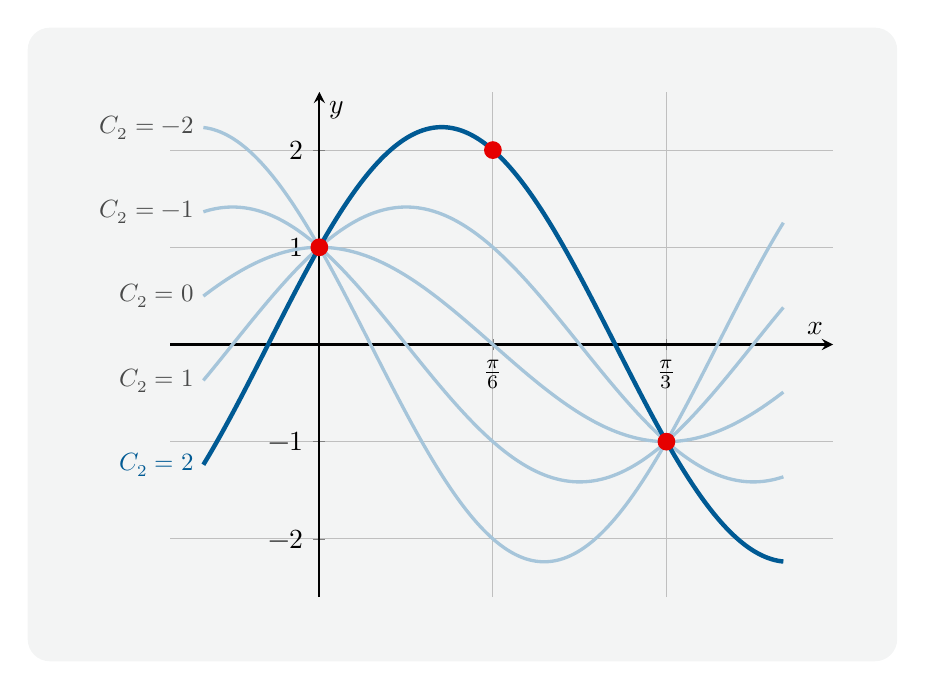
\begin{tikzpicture}[
    show background rectangle,
    background rectangle/.style={fill=my_lightgray, rounded corners=8pt},
    inner frame sep=0.8cm
]
% ---------------------------------------------------------------
%  Loesungen y = cos(3x) + C2 sin(3x) der DGL y'' + 9y = 0 mit y(0) = 1
%  fuer C2 = -2, ..., 2, hervorgehoben C2 = 2 (AWP y'(0) = 6, RWP y(pi/6) = 2).
%  Bei x = pi/6 ist y = C2, bei x = pi/3 ist y = -1 fuer alle C2.
%  Werte bei x = -0.35 (Beschriftung links): 2.232, 1.365, 0.498, -0.370, -1.237.
%  axis equal weggelassen: Bei gleicher Skalierung waere das Bild bei
%  y-Werten von -2.5 bis 2.5 und x-Werten bis 1.4 fast dreimal so hoch wie breit.
% ---------------------------------------------------------------
\begin{axis}[
    axis lines = center,
    xlabel = {$x$},
    ylabel = {$y$},
    grid = both,
    axis line style={thick},
    width=10cm, height=8cm,
    xmin=-0.45, xmax=1.55,
    ymin=-2.6, ymax=2.6,
    xtick={0.5236, 1.0472},
    xticklabels={$\frac{\pi}{6}$, $\frac{\pi}{3}$},
    ytick={-2, -1, 1, 2},
    clip=false,
]
\foreach \C in {-2, -1, 0, 1}{
    \addplot[draw=my_darkblue!35, samples=200, very thick, domain=-0.35:1.4]
        {cos(deg(3*x)) + \C*sin(deg(3*x))};
}
\addplot[draw=my_darkblue, samples=300, ultra thick, domain=-0.35:1.4]
    {cos(deg(3*x)) + 2*sin(deg(3*x))};
\addplot[only marks, mark=*, mark size=3pt, my_red]
    coordinates {(0, 1) (0.5236, 2) (1.0472, -1)};
\node[left, font=\small, my_darkgray] at (axis cs:-0.35, 2.232) {$C_2 = -2$};
\node[left, font=\small, my_darkgray] at (axis cs:-0.35, 1.365) {$C_2 = -1$};
\node[left, font=\small, my_darkgray] at (axis cs:-0.35, 0.498) {$C_2 = 0$};
\node[left, font=\small, my_darkgray] at (axis cs:-0.35, -0.370) {$C_2 = 1$};
\node[left, font=\small, my_darkblue] at (axis cs:-0.35, -1.237) {$C_2 = 2$};
\end{axis}
\end{tikzpicture}
\end{document}
